\section{The replication crisis and meta-analysis}

In the 60s and 70s, there was a big conflict in clinical psychology. On one side were the Freudians, protective of the practice of psycho-dynamic therapy, a therapy based on concepts such as the unconscious and the importance of early life experiences. On the other side were the behaviourists, who mocked Freud's theory as unscientific, and preferred their variant of therapy, one that didn't need to postulate the existence of unobservables such as the unconscious \parencite[Chapter 4]{Wampold2019-fe}. It was against this backdrop the first meta-analysis was done. \textcite{Smith1977-vw} collected all available high-quality evidence on the efficacy of psychotherapies. They used statistical methods to integrate all of it into a whole. The main conclusions of this meta-analysis are still held to be true: 1.) Psychotherapy is an effective treatment and, 2.) there is no difference in effectiveness between different schools of therapy, the so-called \emph{Dodo bird verdict.}

The meta-analysis' competitor is the \emph{narrative review}, where the author uses her own expertise to amalgamate all the evidence she is aware of. The meta-analysis is preferred to a narrative review since it has a greater objectivity. A narrative review gives the author ample freedom to choose which studies to include, how to weigh the different studies, what questions or ideas to focus on and how to frame the results. In addition, a narrative review has no built-in safeguards against the biases of the author -- this allows for \emph{motivated reasoning} \parencite{Kunda1990-ry}, which could severely impact the quality of the review. On the other hand, a properly conducted meta-analysis allows for fewer of these choices. One reason for this is how meta-analysis deals with the protocols for collecting data and conducting analyses, as they should be registered beforehand \parencite{Egger1997-ue}; another is the transparency and replicability of the analysis. Meta-analyses does not allow idiosyncratic choices of how to frame problems, as statistical estimates are in focus. While a narrative review tells a story about a research field, a meta-analysis gives you dry, numerical quantities such as $\widehat{\mu}$ and $\widehat{s}$, quantities that should represent the most current, most objective estimates of the effect size and its standard error. The meta-analysis has been called the \emph{platinum standard of evidence}, playing on the claim that randomized controlled trials represent the gold standard of evidence \parencite{Stegenga2011-zo}.

But there is another, more practical reason to prefer meta-analyses over narrative reviews. When faced with studies numbering a hundred or more, it is a daunting task for any researcher to process the information in all of them without aid. The methods of meta-analysis allows the researcher to process such ``big data'' without suffering from information overload. Some data is especially difficulty to interpret and work with, for instance heterogeneous data, data with covariates, or the otherwise non-standard data. \parencite[][p. 2]{Borenstein2011-yx}

Since the primary results of a meta-analysis are statistics and $p$-values, the results can be interpreted in the same detached way as you would interpret individual studies. And the practical consequences of amalgamating evidence in this way can be dramatic. It can well be that all the published studies on a treatment are inconclusive, with effect sizes going in opposing directions and all $p$-values greater than $0.05$, but a meta-analysis of the exact same studies is definitive, demonstrating a positive effect without reasonable doubt. An example is the meta-analysis of \textcite{cannon_meta-analysis_2006} on the effect on heart attack prevention of high-dose statin therapy compared to standard-dose statin therapy. The meta-analysis covers four studies, where only one has a significant $p$-value. Still, the meta-analysis obtains a highly significant ($p<0.0001$) effect in the desired direction of better response to higher doses. 
\begin{figure}[h]
\noindent \begin{centering}
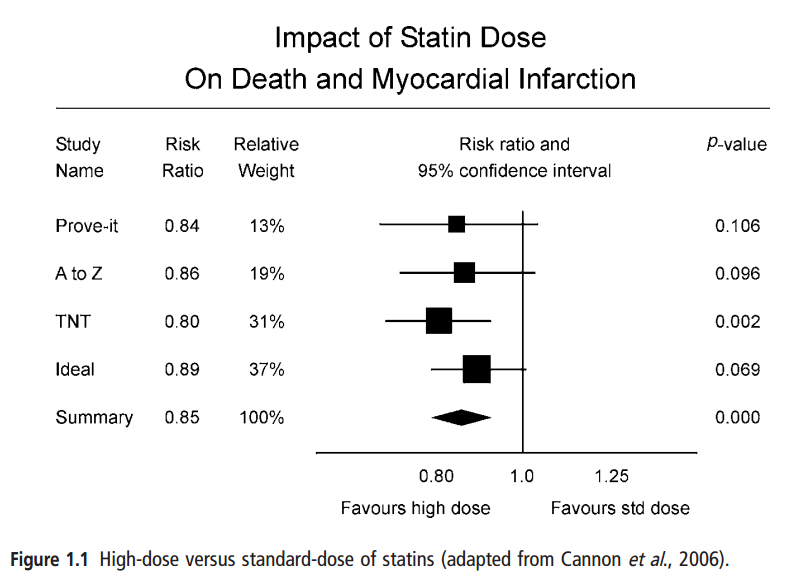
\includegraphics[scale=0.5]{chunks/cannonetal2006}
\par\end{centering}
\caption{\label{fig:A-forest-plot}A \emph{forest plot} of the studies included
in \textcite{cannon_meta-analysis_2006} meta-analysis on statins. The
table is from \textcite[p. 4]{Borenstein2011-yx}.}
\end{figure}
Despite being terribly important, often the difference between life and death\footnote{See the preface of \textcite{Borenstein2011-yx} for a story of how earlier adoption of meta-analyses could have saved the lives of thousands of babies that suffered from sudden infant death syndrome.}, meta-analyses have two weaknesses. The first weakness is subjectivity. For while a meta-analysis is by nature less subjective than a narrative review, it might still be too subjective to settle a scientific question once and for all. This problem is emphasized by \textcite{Stegenga2011-zo}, and is exemplified by the continuing meta-analysis wars in the research on the effect of violent video games on aggressive behavior, as discussed by \textcite{elson_twenty-five_2014}. The other weakness are systematic biases that are hard to model. One of these biases is \emph{publication
bias}, the tendency to publish only positive results. The other is
\emph{p}-hacking, the phenomenon where researchers unconsciously manipulate studies to get small \emph{p}-values.

\subsection{The problems of meta-analysis}
There is a certain degree of subjectivity in any data analysis, and the greater leeway to make subjective choices, the stronger the  tendency for the authors to make self-serving choices. An extreme variant of this is covered by \textcite{Steegen2016-fj}, where it was shown that a study about the combined effect of relationship status and fertility \parencite{Durante2013-yx} could be analyzed in at least 210 different ways. Only some of these gave results in the desired direction and, not surprisingly, the published paper had results in the desired direction as well. 

The meta-analyst must choose which studies to include in her meta-analysis. There is often a good deal of subjectivity here, for it is rarely so that a study is unambiguously eligible for inclusion. There are many reasons to exclude a potential study from a meta-analysis. An oft-discussed bias is \emph{location bias}. If the meta-analysts are English, they will have a hard time incorporating foreign language studies into their meta-analysis \parencite{Egger1998-kj}, resulting in a location-specific meta-analysis. In addition, the meta-analyst will often include only studies from peer-reviewed scientific journals, ignoring studies from dissertations or the gray literature. There are trade-offs involved in the choice of including non-published studies. On one hand, inclusion of unpublished studies might reduce publication bias \parencite{Egger1997-ue}, but it could also increase the bias of the meta-analysis. The bias can increase since the meta-analyst must rely on her network of researchers to obtain the unpublished studies -- but her network is likely to be biased in exactly the same direction as she is. An example of this effect is found in \textcite{Ferguson2010-to}'s discussion of \textcite{Anderson2010-ki}'s meta-analysis on the effect of violent video games on behaviour. The literature on video game violence and aggression is divided into two camps. The camp associated with Anderson holds that violent video games cause aggression, the camp associated with Ferguson holds that they do not. In order for a meta-analysis to be accepted by all camps, it should not be biased against including studies from the opposite camp. However, \textcite{Anderson2010-ki} included several unpublished studies in their meta-analysis, but most were from their own Anderson's group or associated groups.
\begin{quote}
For example, of two unpublished studies, both are from Anderson et
al.'s broader research group. Of three in-press manuscripts
included, two (67\%) are from the Anderson et al. group. Of conference
presentations included, 9 of 12 (75\%) are from the Anderson et al.
group and colleagues. 
\begin{flushright}
-- \textcite[p. 2]{Ferguson2010-to}
\par\end{flushright}
\end{quote}
Another source of subjectivity is whether to only include randomized controlled trials. There is broad agreement that only randomized controlled trials should be included in a meta-analysis if these trials exists \parencite{Egger1997-ue}. The reason is that randomized controlled trials are not affected by confounders in the same way as e.g. case control studies and other observational studies. However, excluding observational studies violates the principle of total evidence, that your conclusions should be based on all available evidence, not just a subset of it, see \textcite{Stegenga2011-zo} for an extended discussion.

A reason to exclude a study is that it does not fulfill a list of best practices. Not all studies are created equal, some are simply of better quality than others. For instance, a subset of studies might have much better measuring instruments than the rest, making it reasonable to include only the studies with the good measuring instrument. But this is yet another source of subjectivity. As an example \parencite[][p. 6]{lakens_reproducibility_2016}, consider the following ``best-practice'' from \textcite{Anderson2010-ki}'s aforementioned meta-analysis on the effect of violent video games  on behaviour. In order to qualify for a best-practice study, the control group must be exposed to a non-violent game, while the treatment group must be exposed to a violent game. One unaccepted treatment-control pair was \emph{Mortal Kombat} vs \emph{Sonic the Hedgehog.} While Mortal Kombat is a fighting game infamous for its violence, Sonic the Hedgehog involves playing a hedgehog jumping on robots, and would easily be classified as among the least violent games by many researchers. On the other hand, an accepted treatment-control pair was \emph{Simpsons Hit \& Run} vs \emph{Grand Theft Auto 3}, even though Simpsons Hit \& Run involves pulling people out of their car in high-speed situations. 

Finally, studies can be excluded since they look suspicious. There are many cases of both reporting errors \parencite{Nuijten2016-eu} and downright fraud in the research literature, with Diedrik Stapel being a high-profile fraudster from social psychology. Since research data is seldom available, the meta-analyst will not be able to check the veracity of the reported results in each research paper. This can lead to exclusion of studies on seemingly ad-hoc grounds. As an example, take \citeauthor{ferguson_angry_2015}'s 2015 meta-analysis on the effect of violent video games on aggressive behaviour. In this analysis, he excluded the study of \textcite{gentile_effects_2009} due to what \textcite{ferguson_angry_2015} called ``bouncing beta'' regression coefficients, or regression coefficients of equal magnitude going in opposite directions, a choice heavily criticized \textcite{gentile_what_2015}.

\subsection{Publication bias and $p$-hacking}

In 1959, \citeauthor{Sterling1959-cq} noted that many journals in psychology only regard an hypothesis as supported if its associated $p$-value was less than $0.05$. Then he hypothesized that this rigid rule would cause that studies with non-significant results not to be published. In order to test this hypothesis, he sampled $364$ papers from four psychology journals and registered the results from the statistical tests contained in them. The result was staggering: Out of $296$ significance tests, only $8$ were non-significant at the $0.05$ level. To account for such an observation without invoking publication bias would require extraordinary assumptions on the ability of psychologists to find real effects. The phenomenon that almost only publications with a $p$-value less than $0.05$ are published is commonly referred to as \emph{publication bias} or the \emph{file-drawer
problem} \parencite{rosenthal_file_1979}.

While the most famous cause of publication bias is the tendency for scientific journals to only accept articles containing statistically significant results, typically at the level of $0.05$ \parencite{simmons_false-positive_2011}, it should be understood more broadly, as the tendency to not publish null-results, or even weak results. The exact mechanism behind publication bias are unknown. For instance, a study reaching ``borderline statistical significance'' or even ``trending towards significance'', with a $p$-value at say $0.07$, is probably somewhat more likely to be published than a study with a $p$-value of $0.23$. If there is evidence for a null-effect, the paper is more likely to be published when the evidence for the null effect is strong, which is the case with large $n$ studies. Still, the cut-off at $p = 0.05$ is conspicuous. 

A cousin of publication bias is \emph{$p$-hacking}, the process of actively changing the data analysis in order to obtain significant results:
\begin{quote}
While collecting and analyzing data, researchers have many decisions to make, including whether to collect more data, which outliers to exclude, which measure(s) to analyze, which covariates to use, and so on. If these decisions are not made in advance but rather are made as the data are being analyzed, then researchers may make them in ways that self-servingly increase their odds of publishing. 
\begin{flushright}
-- \textcite[p. 1]{simonsohn_p-curve:_2014}
\par\end{flushright}
\end{quote}
As emphasized by \textcite{simonsohn_p-curve:_2014}, the presence of $p$-hacking creates bias even when \emph{all} conducted studies are published. In fields such as social psychology, where there is no consensus about how to measure different constructs, which statistical methods to use, or what variables your can condition on, it is almost always possible to get statistically significant result out of your study.\footnote{See \textcite[p. 2, study 2]{simmons_false-positive_2011} for a humorous instance of this, where a literally impossible phenomenon is established with $p<0.05$.} It is even possible to obtain enough results to fill four papers with spurious results, as was the case with food scientist Brian Wasnink \parencite{van_der_zee_statistical_2017}. This newfound focus on $p$-hacking changes how we view publication bias -- for instance, the common-sense claim that ``\emph{when a pattern is seen repeatedly in a field, the association is probably real, even if its exact extent can be debated}\textquotedblright{} (\textcite{ioannidis_why_2008}, cited in \textcite{simonsohn_p-curve:_2014}) is likely to be incorrect. Since $p$-hacking is ubiquitous, it is the popularity of a purported effect which determines the number of published studies on the same or similar effects, not the likelihood of obtaining a significant result.

Publication bias and \emph{p}-hacking are ubiquitous in psychology. A solid piece of evidence for this claim is the study of \textcite{Motyl2017-dx}. They collected all critical effect size estimates and \emph{p}-values from the four top-tier journals \emph{Journal of Personality and Social Psychology}, \emph{Personality and Social Psychology Bulletin}, \emph{Journal of Experimental Social Psychology}, and \emph{Psychological Science}. A critical effect size or \emph{p}-value is one that is used to support the core hypothesis of the paper. That is, the list of statistics does not include statistics associated with auxiliary questions such as ``are there significantly more woman than men in the sample''. These statistics were collected over the pre-replication crisis year
$2003$--$2004$ and the post-replication crisis years $2013$--$2014$. 

Figure \ref{fig:motyl} plots estimated effect sizes from \textcite{Motyl2017-dx} together with the line $y=1.96/\sqrt{n}$, the threshold for significance using the two-sided normal \emph{p}-value. The random effects meta-analysis model yields the estimates $\hat{\mu}_{0}=0.42$ and $\hat{\tau}_{0}=0.34$, Notice how the studies cluster just about threshold for significance, which is extremely unlikely
under normal sampling.
\begin{figure}
\noindent \begin{centering}
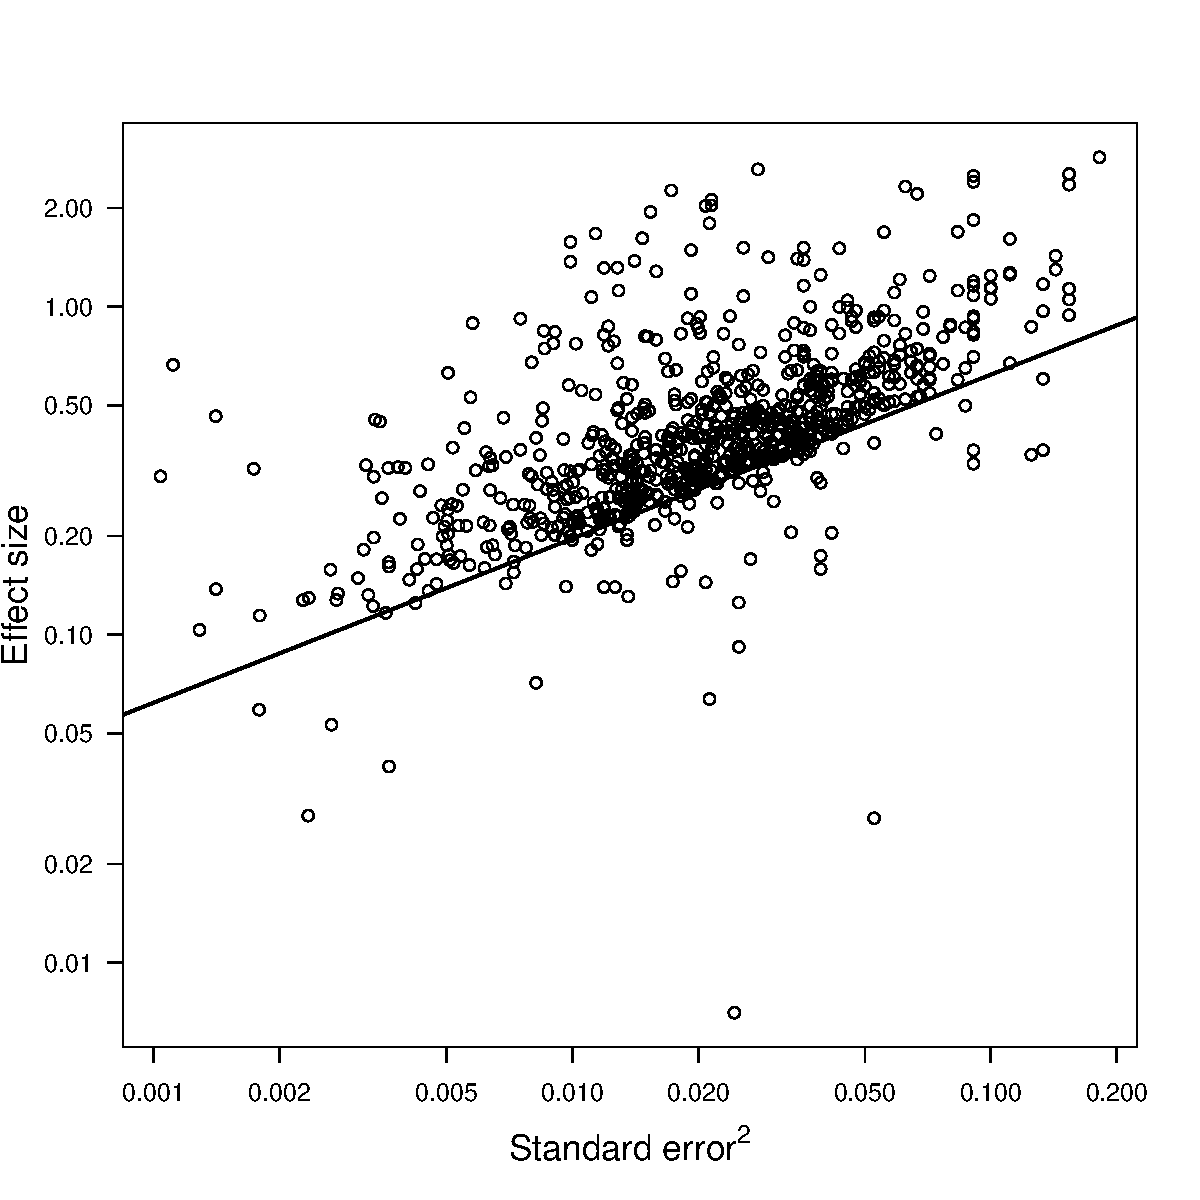
\includegraphics[scale=0.5]{chunks/motyl}
\par\end{centering}
\caption{\label{fig:motyl}Estimated effect sizes and squared standard errors from \textcite{Motyl2017-dx}. The black line is $y=1.96/\sqrt{n}$, the threshold for significance using the two-sided normal \emph{p}-value. Both axes are logarithmic. The number of studies is $n=862$, and the percentage significant results is $91.5\%$.}
\end{figure}
\subsection{Correction for publication bias and $p$-hacking}

There are several methods that attempts to identify and even correct for publication bias. The most widely used is the \emph{funnel plot} of \textcite{Egger1998-kj}, where the standard error of each study is plotted against its effect size. Under severe publication bias, this plot will be skewed. This is because small studies, which will
typically be those with high standard errors, must have large estimated
effect sizes in order to cross the $p=0.05$ boundary. Figure \ref{fig:A-funnel-plot} contains an example of such a plot, based on a subset of the data in the video game and aggression meta-analysis of \textcite{Anderson2010-ki}, and made with the $\mathtt{R}$-package $\mathtt{metafor}$. \parencite{viechtbauer_conducting_2010}.

\begin{figure}
\noindent \begin{centering}
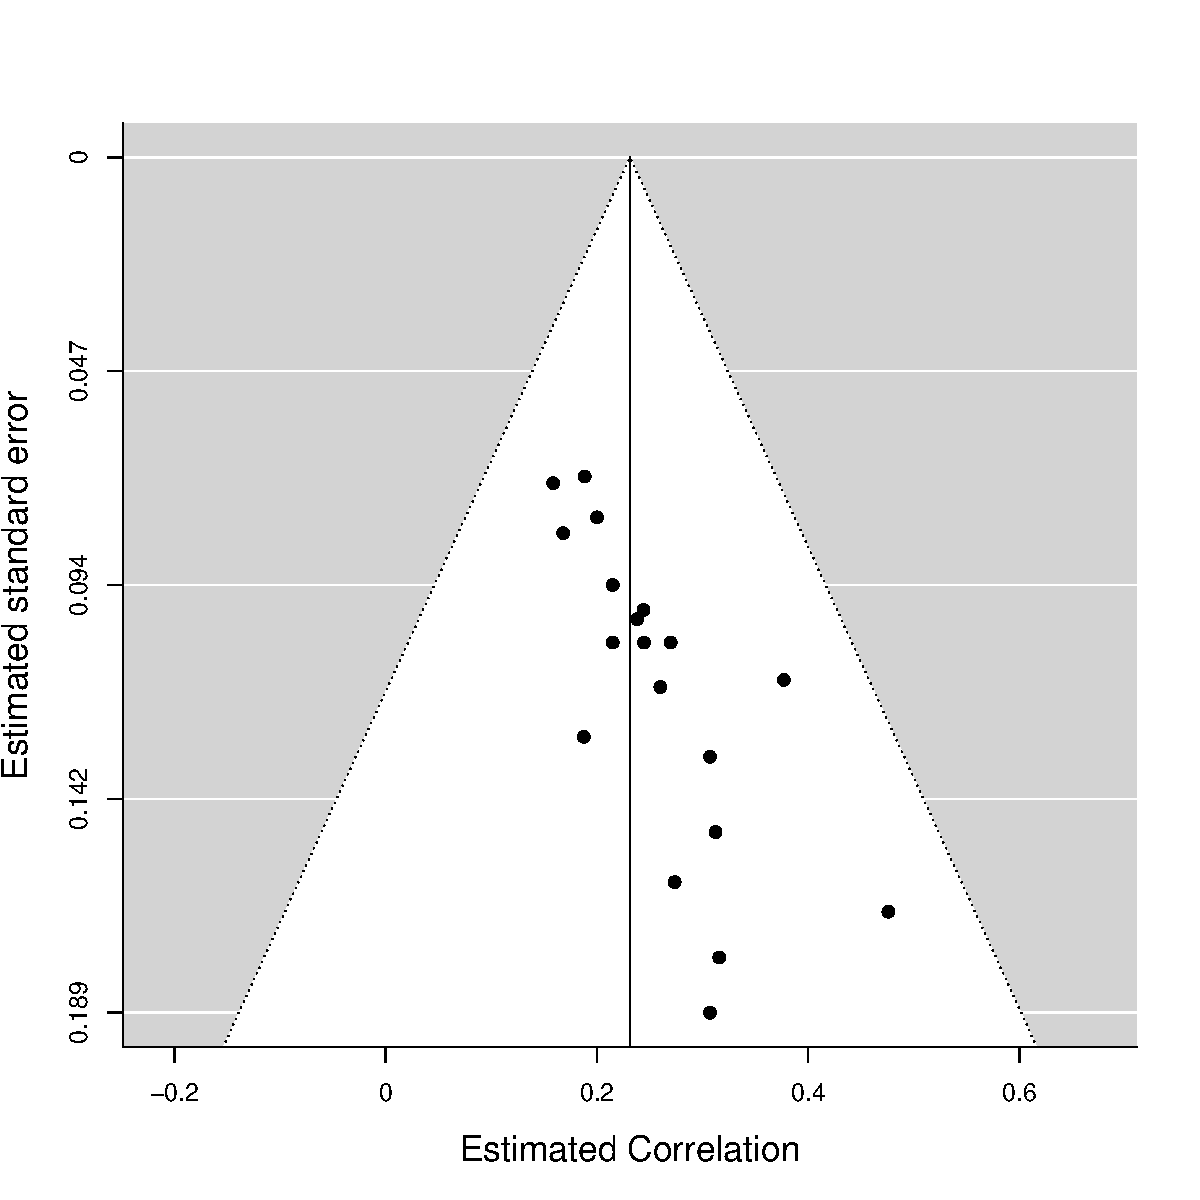
\includegraphics[scale=0.5]{chunks/anderson}
\par\end{centering}
\caption{\label{fig:A-funnel-plot}A funnel plot of a subset from the meta-analysis of \textcite{Anderson2010-ki} on the effect of violent video games on aggressive behavior. The funnel plot is highly skewed to the left, which indicates severe publication bias.}
\end{figure}

Under severe publication bias, this plot will be skewed. Building on this method intuition, the authors propose to estimate a publication bias-corrected effect size by running the regression
\[
x_{i}\sim\theta+\beta\widehat{s}_{i}+\epsilon_{i},
\]
where $\theta$ is the adjusted effect size and $\beta\neq0$ indicates the presence publication bias. This method is called PET \parencite{stanley_beyond_2005}. But PET is not the only regression-based method for publication bias
correction. Another popular method is PET-PEESE \parencite{Stanley2014-gx}, a modified version of the above regression, applied mostly in economics research and recently to psychology \parencite{carter_series_2015}. This method is not without critics. \textcite{gervais_putting_2015} claims the method systematically underestimates the effect size in presence of publication bias, making almost any effect appear to be indistinguishable from $0$. In addition, \textcite{simonsohn_[59]_2017} runs simulations to show that the method fails in presence of inter-study heterogeneity. The most popular method in medicine is named trim and fill \parencite{Duval2000-ct}, which is based on removing and adding non-observed studies to the funnel plot in order to make it symmetric. The $p$-curve of \textcite{simonsohn_p-curve:_2014} has proven to be popular in psychology. This method is based on the theoretical shape (under the null of no $p$-hacking) of the probability density function obtained from the $p$-values from a set of studies.

The theoretically best justified model for publication bias are the selection models, which model publication bias directly using a rejection sampling method \textcite{Hedges1992-ue}. For a simulation study comparing methods to account for publication bias, see \textcite{moreno_assessment_2009,Carter2019-rw}.

All these methods, except the selection models, share a serious shortcoming. Popular statistical methods, such as linear regression and logistic regression, are based on explicitly defined models. These models allows for clear cut estimation of parameters, parameters with univocal definitions and interpretations. The methods for publication bias are not based on explicit models. As such, their estimated quantities are hard to interpret, and are defined in an offhand way. For instance, PET-PEESE is based on one half intuition, one half semi-rigorous mathematics; the $p$-curve of is based on statistical properties of a null-model we assume that is false. 

The meta-analyst will have to make a choice of correcting for publication bias or not. If she opts to correct for publication bias, she is faced with a large number of different methods, most of them not particularly good, but if her choice is no, her resulting estimates might be severely biased. The effect of this choice is potentially tremendous. As an illustration, I take a well-known contentious issue from economics: What is the relationship between the minimum wage and employment? The predictions from economic theory about this are unequivocal: Rising the minimum wage should raise the rate of unemployment. There are two reasons why: First, when the minimum wage is raised above the competitive wage, the employer will shift his spending towards other venues such as capital investments. Second, the industries affected will increase their prices to consumers, reducing the demand for labor in turn. \textcite{doucouliagos_publication_2009} studies the empirical research the relationship between a minimum wage floor and employment. Their meta-analysis contains $64$ studies, which in turn contain a total of $1474$ employment elasticity estimates. The average elasticity was $-0.19$, while the fixed effects meta-analytic estimate was $-0.054$, both highly significant. However, their publication bias-corrected estimate was the meager $-0.01$. In the words of \textcite{doucouliagos_publication_2009}: ``An elasticity of -0.01 has no meaningful policy implications. If correct, the minimum wage could be doubled and cause only a 1 per cent decrease in teenage employment.'' In this case the decision to correct for publication bias reduced the effect size estimate with a factor of $5$. Needless to say, this could have huge policy implication, considering the recent push towards rising the minimum wage in California and other U.S. states \parencite{Lee2016-bd}.

Since publication bias and $p$-hacking is ubiquitous and its effect can make the difference between two radically different conclusions, good methods for dealing with them are needed. Even more important, scientist should rigorous in their usage of methods designed to avoid publication bias and $p$-hacking, for instance study pre-registration. Most importantly, science should be open, transparent, and reproducible. 

\subsection{Open science}

Scientific data is hard to get by request, even for editors. In an editorial for the neuroscience journal Molecular Brain, \textcite{Miyakawa2020-ze} described his experience with asking authors for raw data. Out of the $180$ submissions he handled, he made $41$ requests for raw data as part of a ``Revise before review'' decision. Among these $41$ manuscripts, $21$ withdrew their submission. Out of the $20$ manuscripts left, Miyakawa rejected $19$ due to insufficient raw data. Thus $97\%$ of the submissions failed to provide raw data of good quality even after a request. Miyakawa suggests the possibility ``that the raw data did not exist from the beginning, at least in some portions of these cases.''

Data is even harder to get for non-editors. As part of a study of psychological research's robustness to outliers, \textcite{Wicherts2006-yy} requested data from $141$ research psychologists, but received some data from only $27\%$ percent of them. This was not plausibly because the data was lost: All of the papers they requested data from were published during the last $12$ months. Moreover, the contacted psychologists reneged on their duty. All of them had signed the American Psychological Association's $2001$ ethics code, which contains the sentence ``psychologists do not withhold the data on which their conclusions are based from other competent professionals'' \parencite[p. 396; as cited in Wicherts et al. 2006][]{American_Psychological_Association2001-rs}. 
\textcite{Wicherts2006-yy} are not the only researchers who have had trouble getting data. \textcite[p. 526]{Nelson2018-ov} wrote: 
\begin{quote} Requesting data from another researcher---particularly for the stated justification of suspecting fraud---is socially taxing. Furthermore, although the APA prescribes the sharing of data, there is no enforcement mechanism. We have heard many stories from other researchers who were told that the requested data were coming soon (but then never arrive), were impossible to share, had been lost, or were legally impounded. We have personally been denied data explicitly because the authors wished to avoid criticism; the authors wrote bluntly, \textquotedblleft no data for you.''
\end{quote}
There are some valid reasons not to share data. Most important is the issue of privacy, where there are both ethical and legal issues. But for the majority of psychology papers, the reasons not for sharing data are bad. It is natural to suspect that data is withheld since the authors want to avoid criticism or scrutiny, and there is some evidence for this suspicion. Using the data from the aforementioned study of \textcite{Wicherts2006-yy}, \textcite{Wicherts2011-eb} argue that the reluctance to share data is associated with the study's quality. For instance, $25\%$ of the studies that did not share data reported \textit{p}-values below $0.05$ when they were not, in fact, below $0.05$; this error was not committed by any of the studies that shared data.

The benefits of sharing data are numerous, and not always obvious. \textcite{Wicherts2012-cp} lists six points. First, sharing data preserves it. If you keep your data only on your own computer, it will eventually be lost. Second, openness allows other researchers to independently reproduce your results. They can uncover errors in the analysis, \emph{p-}hacking, or scientific misconduct. Third, publishing data can make the paper more citeable. This is especially relatable for methodologists, who frequently cite papers only since they are associated with data sets. Fourth and fifth, other researchers can run different analysis on your data. For statisticians this one is an obvious one, and is especially important for meta-analysists \parencite{Cooper2009-ge}. Finally, founding agencies routinely stipulate that data must kept in an accessible form for some minimum amount of years. If the data are made open, you do not have to worry at all about this.  

A major reason to demand open data is to prevent scientific fraud. While most researchers believe that fraud is uncommon, it is extremely difficult to measure. Since there are strong incentives to falsify data and incorrectly report summary statistics, it is imprudent to assume no one does it. Demanding open data reduces the number of fraudulent papers by two mechanism. First, you are strongly disincentivized to falsify data and summary statistics when the data are publicly available. For other researchers can, in principle, uncover your fraud at any moment. Second, fraudulent papers will be uncovered at a greater rate when the evidence is available for scrutiny. By merely looking at reported standard deviations and means, \textcite{Simonsohn2013-ul} started to suspect two authors of systematic data manipulation. Luckily, the authors supplied him with the raw data, which only strengthened the suspicion of fraud. One of the authors, Dirk Smeesters, has now been convicted of scientific misconduct. The other, Lawrence Sanna, suddenly resigned from his professorship. However, \textcite{Simonsohn2013-ul}
also observed a ``third case of exceedingly similar summary statistics''. Sadly, he did not get hold of the data, as the ``main author reported losing them, and the coauthors of the article did not wish to get involved''.

%Sharing data is just one part of open and reproducible science. It is equally important to share the code employed in the preparation of the manuscripts. The code should be readable, that is, no spaghetti code, documented, and preferably tested. Even better, the code should be integrated with the manuscript itself, allowing a compilation of a single file to reproduce the entire manuscript. The $\mathtt{R}$ environment provides tools to do such reproducible science, most importantly \texttt{rmarkdown} \parencite{Xie2018}.

%The reasons to share code are pretty much the same as the reasons to share data. Openness fosters better research and invites scrutiny for other researchers. It increases the trust in your research. It probably fosters collaboration too; it is much easier to approach someone about what they do when you know what they are doing.

%Papers report inconsistent statistics. \textcite{Nuijten2016-eu} reports that one of two psychology papers contains \emph{p}-values that are inconsistent with its reported test statistics. Moreover, one of eight papers have gross inconsistencies, where a reported \emph{p}-value is significant but its computed \emph{p}-value is not. As a reader without access to either the data or the code used to calculate the statistics, you are left in the dark about what the data actually says.

\textcite{John2012-xp} measured the frequency of \emph{p}-hacking and other questionable research practices, in psychology using an electronic survey. Figure \ref{fig:john2012} shows their results. Most of these questions are about \emph{p}-hacking, but question eight is about \emph{hypothesising after results are known} (denoted \emph{HARKing} by \textcite{Kerr1998-by}), and question ten about scientific fraud. Approximately one third of the respondents admitted to hypothesising after results are known. Doing this certainly makes \emph{p}-values invalid, as choosing a null hypothesis conditioned its \emph{p}-value being less than $0.05$ definitely makes you reject the null hypothesis. But hypothesising after results are known is detrimental for other reasons too, and \textcite[p. 205]{Kerr1998-by} lists nine additional reasons why.

\begin{figure}
\noindent \begin{centering}
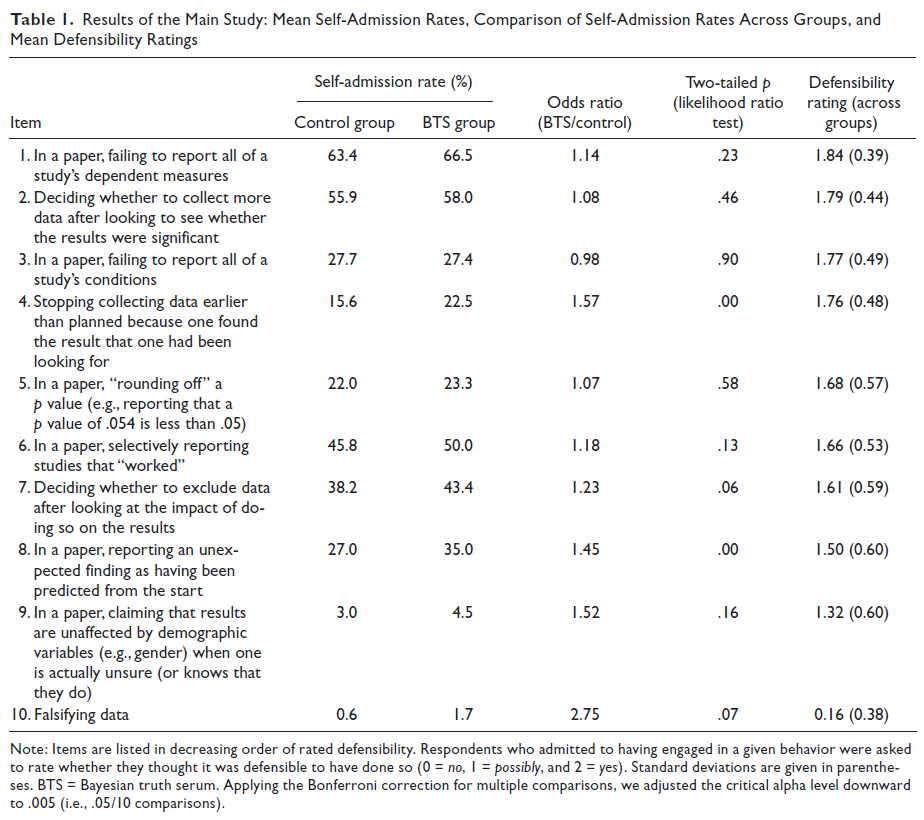
\includegraphics[scale=0.4]{chunks/john2012}
\par\end{centering}
\caption{\label{fig:john2012}Self-admission rates to questionable research practices from \textcite{John2012-xp}. The participants in BTS group were given incentives for honest reporting, and the defensibility rating indicates how defensible the respondents consider each practice to be.}
\end{figure}

A study is preregistered if it is planned in detail in advance and the this plan is publicly known \parencite{Van_t_Veer2016-fo}. The plan should include the what hypotheses are tested, the experimental methods used, and an exact specification on the statistical analysis. A benefit of proper preregistration is that it makes hypothesising after results are known impossible, which on its own should reduce the rate of false positives in the literature quite a bit. But preregistration is also a remedy for \emph{p}-hacking, and can even help with publication bias.

\textcite{Scheel2020-sq} studied rate of positive results in standard research versus preregistered research. Among $148$ standard, non-preregistered studies sampled, $142$ were positive. That is, $95\%$ were positive. On the other hand only $15/30=50\%$ of the preregistered reports were positive. Such a rate of positive results is far more plausible than $95\%$, especially when seen in light of the fact that most psychological research is severely underpowered \parencite{Sedlmeier1989-zz}.

\subsection{Back-of-the-envelope calculations }
A large part the daily lives of researchers is spent on reading and critically engaging with other peoples research. Prior to the replication crisis, a common way to judge the worth of an effect was to look at its \emph{p}-value or \emph{t-}value. If the \emph{p}-value was smaller than $0.05$, or the \emph{t-}value larger than approximately $2$, results looked impressive enough to be worthy of consideration. While plenty of researchers believe this way to consume research is bad \parencite{Gigerenzer2004-oc}, it is not without its merits. We have limited attention spans and need to abide by some decision rules; what we need are well-justified decision rules that will not lead us astray with an unacceptably high probability.

Making a couple of half-plausible assumptions, there are some simple ways to correct isolated studies for publication bias and \emph{p}-hacking. We will take a short look at two back-of-the-envelope methods, one for expectations and one for effect sizes. Both are based on a simple model of selection for significance, where we observe only significant normal $X$s. Assume $X\sim N(\mu,n^{-1/2})$ and let $U=\Phi(-n^{1/2}X)$ be the standard one-sided $p$-value. 

Let's have a look at the corrected expectation first. The expectation of the left-truncated normal is \parencite[Section 10.1]{Johnson1994-ag}
\begin{equation}
\mu+\sigma M'\left(\frac{a-\mu}{\sigma}\right),\label{eq:mean of truncated normal}
\end{equation}
where
$M'(\text{\ensuremath{\theta}})=\phi(\text{\ensuremath{\theta}})/\Phi(-\text{\ensuremath{\theta}})$
is the inverse Mills' ratio. 
In our case, $a=c_{\alpha}n^{-1/2}$ and $\sigma=n^{-1/2},$ and the expectation equals $\mu+n^{-1/2}M'(c_{\alpha}-n^{1/2}\mu)$, where $c_\alpha = \Phi^{-1}(1-\alpha)$. When
$\mu=0$ and $\alpha=0.05$, we get $E(X\mid n^{1/2}X>c_{\alpha})=n^{-1/2}\alpha^{-1}\phi(c_{\alpha})\approx2n^{-1/2}.$
This value is easy to remember and compute, and provides a realistic baseline to compare effect sizes against. In a world free of biases, we would informally compare an effect size against $0$. In a world with publication bias and \emph{p}-hacking, comparing against $2n^{-1/2}$ is smarter and almost as easy. From the data set of \textcite{Motyl2017-dx} we just looked at, we get $2\overline{n^{-1/2}}=0.24$. That is, we would expect a mean effect size of $0.24$ from psychology even when the true mean is $0$, assuming complete selection for significance and the validity of the normal approximation. The actual mean of the data set, $\overline{\theta}=0.45$, does not look that impressive anymore.

There are strong reasons not to care only about \emph{p}-values, but also about effect sizes \parencite{Funder2019-tg}. The natural way to
estimate the effect size $\mu$ is to use the maximum likelihood estimator $\hat{\mu}$. While this quantity is easy to calculate numerically, it is hardly convenient to use when reading a paper. Luckily, there are simple bounds for the maximum likelihood estimator.
\begin{proposition}
\label{prop:maximum likelihood bounds}The maximum likelihood estimator of $d$, called $\hat{d}$, based on a single observation $x$ from a study with $n$ participants is bounded by 
\[
l(x)\leq\hat{d}(x)\leq u(x).
\]
The bounds are equal to
\begin{eqnarray}
l(x) & = & x-\frac{1}{n^{1/2}\delta},\label{eq:lower bound}\\
u(x) & = & x-\frac{1}{n^{1/2}\delta}\max\{1-\delta^{2},0\}.\label{eq:upper bound}
\end{eqnarray}
where $\delta=n^{1/2}x-\Phi^{-1}(1-\alpha)$.
\end{proposition}

You could argue that $\delta$ does not look that simple to work with, but it is. For $n^{1/2}x$ is the \textit{t}-value, which is often reported in the paper itself. The value of $\Phi^{-1}(1-\alpha)$, on the other hand, equals $1.96$. It might be profitable to increase it slightly, to e.g. $2$, to account for the fact that \textit{t}-tests are frequently used. Now $n^{1/2} - \Phi^{-1}(1-\alpha) \approx t - 2$, which is easy to calculate by hand. If $1/(t - 2)$ value is too big compared with $n^{1/2}$, you can probably disregard the study. 

Consider Study 1 of the infamous \emph{power posing} paper by \textcite{Carney2010-we}. Here $t = 2.07$, so that $1/(t - 2) \approx 14$ with $38$ degrees of freedom. Since $38^{1/2} \approx 6$, we see that $1/(t - 2)$ is much larger than $38^{1/2}$, and we can probably ignore the study.

Proposition \ref{prop:maximum likelihood bounds} is a straight-forward
corollary of the following proposition. 
\begin{proposition}
\label{prop:ml bouds}Let $X_{1},\ldots,X_{N}$ be independent samples
from a left-truncated normal. Assuming known truncation point $a$
and standard deviation $\sigma$, the maximum likelihood estimator
$\hat{\mu}$ of $\mu$ is bounded by
\begin{equation}
\overline{x}-\frac{\sigma^{2}}{\overline{x}-a}<\hat{\mu}<\overline{x}-\max\left(\frac{\sigma^{2}}{\overline{x}-a}-(\overline{x}-a),0\right).\label{eq:ml bounds}
\end{equation}
\end{proposition}
\begin{proof}
Differentiating the logarithm of the density of a truncated normal,
we find that the maximum likelihood estimator is the solution to $\mu=\overline{x}-\sigma M'([a-\mu]/\sigma)$. The inverse Mills' ratio can be bounded
elementary functions \parencite{Yang2015-pa}. In particular, it can be
bounded by \parencite[Equation 32]{Gasull2014-hn}
\begin{equation}
M_{u}(\theta)=\frac{1}{2}(\sqrt{\text{\ensuremath{\theta}}^{2}+4}+\text{\ensuremath{\theta}})>M'(\text{\ensuremath{\theta}}),\label{eq:Mills' ratio inequality}
\end{equation}
and 
\begin{equation}
M'(\text{\ensuremath{\theta}})>\frac{1}{4}(\sqrt{\text{\ensuremath{\theta}}^{2}+8}+3\text{\ensuremath{\theta}})=M_{l}(\theta)>\theta.\label{eq:Mill's ratio inequality (2)}
\end{equation}
The functions $M(\text{\ensuremath{\theta}})$ in these inequalities
are increasing in $\text{\ensuremath{\theta}}$, hence $\overline{x}-\sigma M([a-\mu]/\sigma)$
is icreasing in $\mu$. Assume $\mu_{u}$ satisfies $\mu_{u}=\overline{x}-\sigma M_{u}([a-\mu_{u}]/\sigma)$.
Since $M_{u}(\theta)>M'(\theta)$, we have $\overline{x}-\sigma M'([a-\mu_{u}]/\sigma)<0$
too, thus $\mu_{u}<\hat{\mu}$. Likewise, if $\mu_{l}$ satisfies
$\mu_{l}=\overline{x}-\sigma M_{l}([a-\mu_{l}]/\sigma)$, then $\mu_{l}>\hat{\mu}$.
Now define $l(\overline{x})=\mu_{u}$ and $u(\overline{x})=\mu_{l}$.
Now, to find $l(\overline{x})$, solve
\[
\mu=\overline{x}-\sigma\frac{1}{2}\left(\sqrt{\text{\ensuremath{([a-\mu]/\sigma)}}^{2}+4}+\text{\ensuremath{[a-\mu]/\sigma}}\right)
\]
to get $\mu=\overline{x}-\sigma^{2}/(\overline{x}-a)$. The upper
bound $u(\overline{x})$ can be found in the same manner, using both
the lower bounds $M_{l}(\theta)$ and $\theta$ and choosing the best
option.
\end{proof}